\documentclass[a4paper,12pt]{report}
\usepackage{amssymb}

\usepackage{ucs}
\usepackage[utf8x]{inputenc} % Input encoding for Greek characters
\usepackage[greek,english]{babel} % Language support

\newcommand{\en}{\selectlanguage{english}}
\newcommand{\gr}{\selectlanguage{greek}}

% \usepackage{algorithm2e}
% \usepackage{algorithm}
% \usepackage{algorithmic}
\usepackage{enumitem}
\usepackage{tcolorbox}
\tcbuselibrary{listingsutf8}
\usepackage{float}
\usepackage{amsmath}
\usepackage{graphicx} % For including images
\usepackage{titlesec} % Custom title formatting
\usepackage{fancyhdr} % For custom headers and footers
\usepackage{geometry} % For adjusting page margins

% Adjust the page margins to make content wider
\geometry{top=2.5cm, bottom=2.5cm, left=2.5cm, right=2.5cm}

% Redefine chapter formatting to make it smaller
\titleformat{\chapter}[display]
    {\normalfont\LARGE\bfseries} % Smaller size and bold for chapter heading
    {\chaptername\ \thechapter} % Chapter number format
    {15pt} % Space between chapter number and title
    {\bfseries} % Smaller size and bold for chapter title
\begin{document}

\begin{titlepage}
    \centering
    \vspace*{-3cm}
    % University logo
    \includegraphics[width=1\textwidth]{auth_logo.png} % Replace with your actual logo file

    % University name in Greek
    \textbf{\gr ΑΡΙΣΤΟΤΕΛΕΙΟ ΠΑΝΕΠΙΣΤΗΜΙΟ ΘΕΣΣΑΛΟΝΙΚΗΣ}
    \vspace{2cm}

    % Document title and subtitle in Greek
    \LARGE\textbf{\gr Ρομποτική Αναφορά} \\
    \Large\normalfont{\gr Εργασία Τμήμα Α και Τμήμα Β} \\
    \vspace{4cm}

    \gr
    \large
    \textbf{Διακολουκάς Δημήτριος} \\
    \textbf{AEM 10642}
    \vspace{2.5cm}

    \en
    \textit{Email: ddiakolou@ece.auth.gr}
\end{titlepage}

\gr
\tableofcontents

\chapter{Εργασία Ρομποτικής: Τμήμα Α}

\section{Εισαγωγή και περιγραφή του προβλήματος}

Στο πλαίσιο της παρούσας εργασίας ζητείται η προσομοίωση της κίνησης ανοίγματος μιας πόρτας με τη βοήθεια τροχιάς που περιγράφει την κίνηση του πόμολου \en (handle) \gr. Η πόρτα βρίσκεται σε δωμάτιο και περιστρέφεται γύρω από κατακόρυφο άξονα στο σημείο μεντεσέ \en (hinge) \gr, με αρχική θέση πλήρως κλειστή. Στην επιφάνεια της πόρτας υπάρχει τοποθετημένο ένα πλαίσιο \en $\{H\}$ \gr, το οποίο αντιστοιχεί στο πόμολο και περιγράφεται μέσω ενός ομογενούς μετασχηματισμού \en (homogeneous transformation) \gr.

Η διαδικασία ανοίγματος της πόρτας περιλαμβάνει δύο διαδοχικά στάδια:
\begin{itemize}
    \item Περιστροφή του πόμολου κατά $-45^\circ$ γύρω από τον τοπικό άξονα \en $x_h$ \gr με μηδενική αρχική και τελική ταχύτητα και επιτάχυνση.
    \item Περιστροφή της πόρτας κατά $-30^\circ$ γύρω από τον κατακόρυφο άξονα \en $z_d$ \gr, ενώ το πόμολο κινείται συγχρονισμένα ώστε να διατηρηθεί η σχετική του θέση.
\end{itemize}

\hspace{-0.6cm}Η συνολική διάρκεια της κίνησης είναι \en $T = 5$ sec \gr, ενώ στόχος είναι η δημιουργία ομαλής τροχιάς θέσης και προσανατολισμού για το πλαίσιο \en $\{H\}$ \gr. Για την υλοποίηση χρησιμοποιήθηκε το \en Robotics Toolbox \gr του \en Peter Corke \gr στο \en MATLAB \gr, αξιοποιώντας τις συναρτήσεις \en \texttt{tpoly} \gr και \en \texttt{trplot} \gr για χρονική παρεμβολή και τρισδιάστατη απεικόνιση πλαισίων αντίστοιχα.

\hspace{-0.6cm}Η έξοδος της διαδικασίας αποτελείται από δύο πίνακες τροχιάς, τον $g_{oh}$ για το πόμολο \en (handle) \gr $\ge$ και τον $g_{od}$ για την πόρτα \en (door)\gr. Αυτοί οι πίνακες περιγράφουν τη χρονικά εξαρτώμενη θέση και προσανατολισμό των αντίστοιχων αντικειμένων στο χώρο, και θα χρησιμοποιηθούν στο Τμήμα B της εργασίας για την υλοποίηση και αξιολόγηση της αντιστροφικής κινηματικής.

\vspace{0.3cm}

\section{Περιγραφή υλοποίησης σε \en MATLAB \gr}

Ο κώδικας ακολουθεί τα βήματα της περιγραφής και είναι χωρισμένος σε τμήματα:
\begin{itemize}
    \item Ορισμός γεωμετρικών παραμέτρων πόρτας και πόμολου.
    \item Δημιουργία των γωνιακών προφίλ \en $\alpha(t)$ \gr (στρέψη πόμολου) και \en $\beta(t)$ \gr (γωνία ανοίγματος πόρτας).
    \item Υπολογισμός των ομογενών μετασχηματισμών \en $g_{od}(t)$ \gr και \en $g_{oh}(t)$ \gr.
    \item Γραφική απεικόνιση σε κάθε χρονικό βήμα και αποθήκευση των τροχιών.
\end{itemize}

\hspace{-0.6cm}Ο κώδικας διασφαλίζει ρυθμό δειγματοληψίας \en $dt = 0.01$ sec \gr (δηλαδή 100\en Hz\gr), με συνολικά $n = 501$ δείγματα, διατηρώντας ακρίβεια και ομαλότητα της τροχιάς. Η χρήση \en \texttt{UnitQuaternion} \gr επιτρέπει την απεικόνιση της προσανατολισμού του πλαισίου \en $\{H\}$ \gr στον χρόνο.

\vspace{0.3cm}

\section{Ενδελεχής ανάλυση κώδικα και μεθοδολογίας}

Το σύστημα που προσομοιώνεται αποτελείται από μία πόρτα \en (door) \gr η οποία περιστρέφεται γύρω από κατακόρυφο άξονα \en (hinge) \gr και έναν μηχανισμό πομόλου \en (handle) \gr τοποθετημένο επάνω της, που στρέφεται γύρω από το δικό του τοπικό άξονα. Η χρονικά εξελισσόμενη κίνησή τους περιγράφεται μέσω ομογενών μετασχηματισμών του χώρου $\mathrm{SE}(3)$.

\vspace{0.2cm}

\subsection{Γεωμετρική περιγραφή και χρονικά διαστήματα}

Οι βασικές παράμετροι του συστήματος είναι:

\begin{itemize}
    \item $l = 1.0~\mathrm{m}$: πλάτος πόρτας
    \item $lo = 0.1~\mathrm{m}$: απόσταση του πομόλου από τον μεντεσέ
    \item $h = 0.7~\mathrm{m}$: ύψος τοποθέτησης του πομόλου
    \item $door\_height = 2.0~\mathrm{m}$: συνολικό ύψος πόρτας
\end{itemize}

\hspace{-0.6cm}Η χρονική διάρκεια της προσομοίωσης είναι $T = T_1 + T_2 = 5~\mathrm{s}$, όπου $T_1 = 2~\mathrm{s}$ αφιερώνεται στη στρέψη του πομόλου και $T_2 = 3~\mathrm{s}$ στο άνοιγμα της πόρτας καθώς ορίσαμε \en N1 = 201 \gr και \en N2 = 300 \gr καρέ για δειγματοληψία στα \(dt = 0.01\) \en sec\gr.

\vspace{0.2cm}

\subsection{Κατασκευή τροχιών \en (Trajectory Planning) \gr}

Χρησιμοποιείται η συνάρτηση \texttt{\en tpoly \gr} για την παραγωγή λείων, συνεχών τροχιών για τις γωνίες:

\begin{itemize}
    \item $\alpha(t)$: περιγράφει τη στροφή του πομόλου γύρω από τον τοπικό άξονα $x$, αρχικά από $0^\circ$ σε $-45^\circ$ κατά $T_1$ και επιστρέφει στο $0^\circ$ στο $T_2$.
    \item $\beta(t)$: δηλώνει τη στροφή της πόρτας γύρω από τον άξονα $z$, η οποία πραγματοποιείται μόνο στο διάστημα $[T_1, T]$ και φτάνει τα $30^\circ$.
\end{itemize}

\hspace{-0.6cm}Οι τροχιές είναι κατασκευασμένες ώστε να είναι χρονικά ομαλές και μη απότομες, κατάλληλες για εφαρμογή σε ρομποτικά συστήματα.

\begin{figure}[H]
    \centering
    \includegraphics[width=0.7\textwidth]{Initial_pic.png}
    \caption{Αναπαράσταση σχήματος πόρτας και πομόλου με τα πλαίσια \{0\}, \{D\}, \{H\} και τις γεωμετρικές παραμέτρους $l$, $lo$, $h$}
    \label{fig:door_ref}
\end{figure}

\vspace{0.2cm}

\subsection{Κινηματική μοντελοποίηση}

Το πρόβλημα επιλύεται κινηματικά μέσω συνδυασμού στοιχειωδών μετασχηματισμών του χώρου $\mathrm{SE}(3)$. Οι σχετικές θέσεις της πόρτας και του πομόλου εκφράζονται αναλυτικά:

\paragraph{Πόρτα ως προς παγκόσμιο σύστημα:}

Η πόρτα θεωρείται προσαρτημένη σε σταθερό σημείο $(0, 2, 0)$, όπου και βρίσκεται ο άξονας περιστροφής (μεντεσές):

\[
T_{D0}(t) = \text{\en transl\gr}(0,2,0) \cdot \text{\en Rot\gr}_z\big(\beta(t)\big)
\]

\paragraph{Πομόλο ως προς πόρτα:}

Η θέση του πομόλου καθορίζεται από μετατόπιση σε απόσταση $(l - lo)$ κατά τον άξονα $x$ και ύψος $h$, στροφή κατά $-90^\circ$ στον άξονα $z$ για ευθυγράμμιση και εν συνεχεία στρέψη κατά $\alpha(t)$ στον άξονα $x$:

\[
T_{HD}(t) = \text{\en transl\gr}(l - lo, 0, h) \cdot \text{\en Rot\gr}_z\left(-\frac{\pi}{2}\right) \cdot \text{\en Rot\gr}_x\big(\alpha(t)\big)
\]

\paragraph{Πομόλο ως προς παγκόσμιο σύστημα:}

Ο συνολικός μετασχηματισμός για το πομόλο υπολογίζεται ως:

\[
T_{H0}(t) = T_{D0}(t) \cdot T_{HD}(t)
\]

\hspace{-0.6cm}Ο πίνακας $T_{H0}(t) \in \mathrm{SE}(3)$ περιέχει την πλήρη πληροφορία για τη θέση και τον προσανατολισμό του πομόλου σε κάθε χρονική στιγμή.

\vspace{0.2cm}

\subsection{Ανάλυση τροχιάς}

Από τον πίνακα $T_{H0}(t)$ εξάγονται:

\begin{itemize}
    \item $p_h(t) = T_{H0}(t)[1:3,\,4]$: τρισδιάστατη θέση πομόλου
    \item $q_h(t) = \text{\en UnitQuaternion\gr}(T_{H0}(t))$: προσανατολισμός σε μορφή μοναδιαίου τεταρτογωνίου
\end{itemize}

\hspace{-0.6cm}Αυτά τα δεδομένα αποτελούν την έξοδο της προσομοίωσης και εισάγονται στην αντιστροφή κινηματικής.

\vspace{0.2cm}

\subsection{Μαθηματική απεικόνιση του προβλήματος}

Η κινηματική περιγραφή του συστήματος συνοψίζεται στην εξής εξίσωση:

\[
T_{H0}(t) =
\underbrace{\text{\en transl\gr}(0,2,0)}_{\text{μεντεσές}} \cdot
\underbrace{\text{\en Rot\gr}_z(\beta(t))}_{\text{πόρτα}} \cdot
\underbrace{\text{\en transl\gr}(l - lo, 0, h)}_{\text{θέση πομόλου}} \cdot
\underbrace{\text{\en Rot\gr}_z\left(-\frac{\pi}{2}\right)}_{\text{ευθυγράμμιση}} \cdot
\underbrace{\text{\en Rot\gr}_x(\alpha(t))}_{\text{στρέψη}}
\]

\hspace{-0.6cm}Η τροχιά $T_{H0}(t)$ ανήκει στον χώρο $\mathrm{SE}(3)$ και χρησιμοποιείται σε συνδιασμό με την $T_{D0}(t)$ ως αναφορά για τον σχεδιασμό της \en inverse kinematics \gr στο Τμήμα B της εργασίας.

\vspace{0.3cm}

\section{Παρατηρήσεις και Αποτελέσματα}

Στην παρούσα ενότητα παρουσιάζονται και αναλύονται τα αποτελέσματα της προσομοίωσης με βάση τα δεδομένα τροχιάς και τα αντίστοιχα διαγράμματα.

\vspace{0.2cm}

\subsection{Στιγμιότυπα Κίνησης Πόρτας και Πομόλου}

Τα παρακάτω στιγμιότυπα δείχνουν την εξέλιξη του συστήματος σε κρίσιμες χρονικές στιγμές:

\begin{figure}[H]
    \centering
    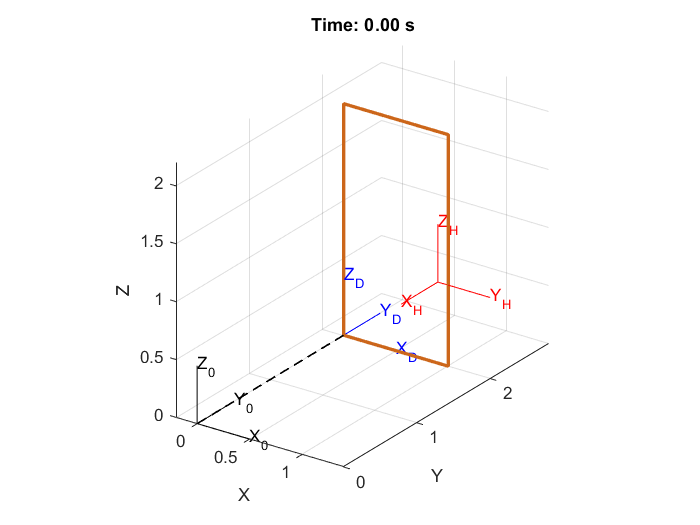
\includegraphics[width=0.48\textwidth]{PartA_First.png}
    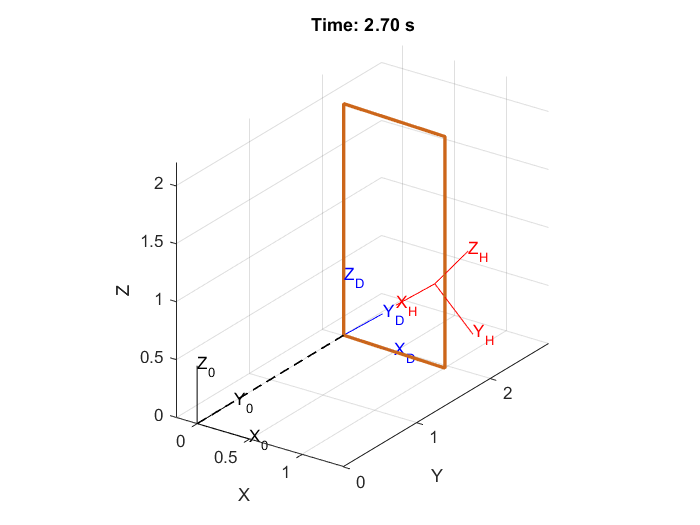
\includegraphics[width=0.48\textwidth]{PartA_Second.png}
    \caption{Αριστερά: \en t = 0.00s \gr (κλειστή πόρτα, αρχή στρέψης). Δεξιά: \en t ≈ 2.7s \gr (τέλος στρέψης, κατά \en 0.7s \gr αρχή ανοίγματος).}
\end{figure}

\begin{figure}[H]
    \centering
    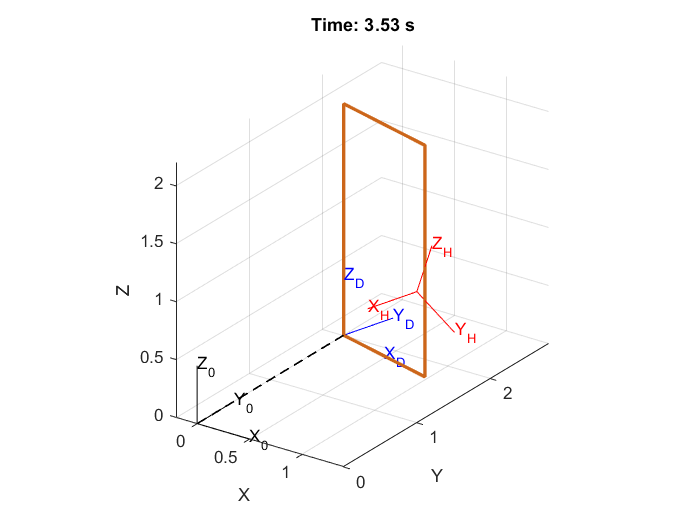
\includegraphics[width=0.48\textwidth]{PartA_Third.png}
    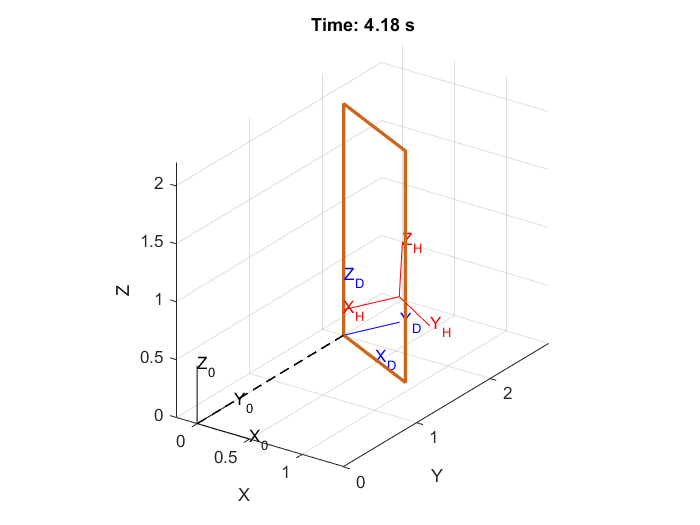
\includegraphics[width=0.48\textwidth]{PartA_Fourth.png}
    \caption{Αριστερά: \en t ≈ 3.5s\gr. Δεξιά: \en t ≈ 4.2s\gr. Παρατηρείται σημαντική περιστροφή της πόρτας.}
\end{figure}

\begin{figure}[H]
    \centering
    \includegraphics[width=0.48\textwidth]{PartA_Fifth.png}
    \caption{Τελική φάση κίνησης με πόρτα πλήρως ανοιχτή \en t = 5s \gr και πομόλο επανελθόν στη θέση ισορροπίας.}
\end{figure}

\vspace{0.2cm}

\subsection{Διαγράμματα για Οπτικοποίηση Μοντέλου Κίνησης}

\begin{figure}[H]
    \centering
    \begin{minipage}{0.48\textwidth}
        \centering
        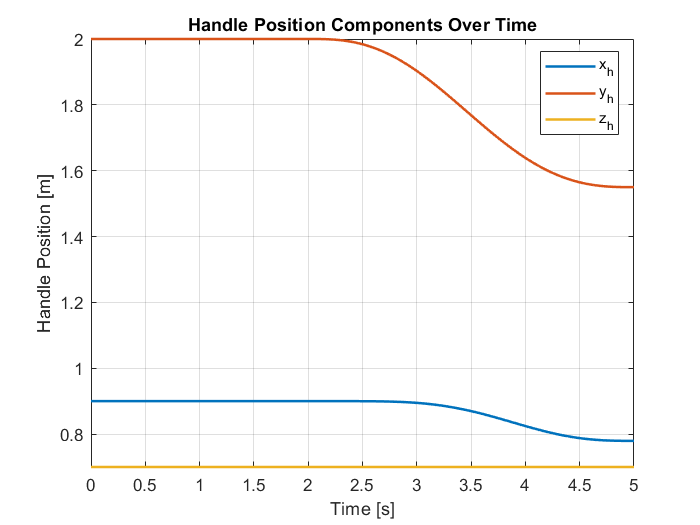
\includegraphics[width=\linewidth]{Handle_Position_Part_A.png}
        \caption{Θέση πομόλου $x_h$, $y_h$, $z_h$ ως προς τον χρόνο.}
        \label{fig:handle_pos}
    \end{minipage}
    \hfill
    \begin{minipage}{0.48\textwidth}
        \centering
        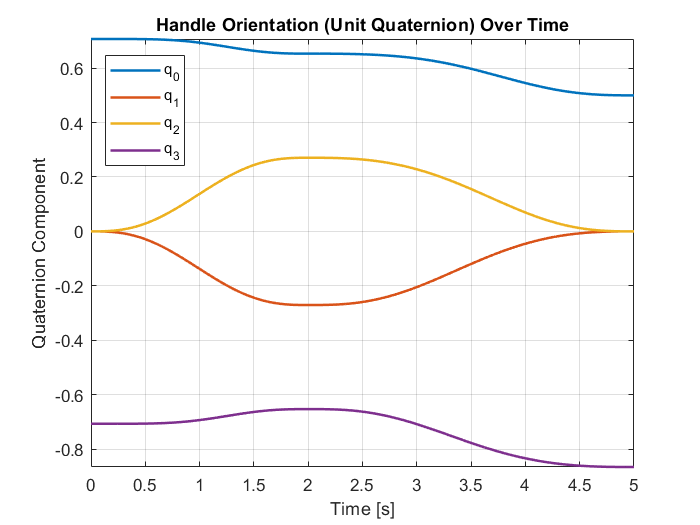
\includegraphics[width=\linewidth]{Handle_Quaternion_PartA.png}
        \caption{Συνιστώσες του μοναδιαίου τεταρτογωνίου $q_0$ έως $q_3$.}
        \label{fig:handle_quat}
    \end{minipage}
\end{figure}

\begin{figure}[H]
    \centering
    \begin{minipage}{0.48\textwidth}
        \centering
        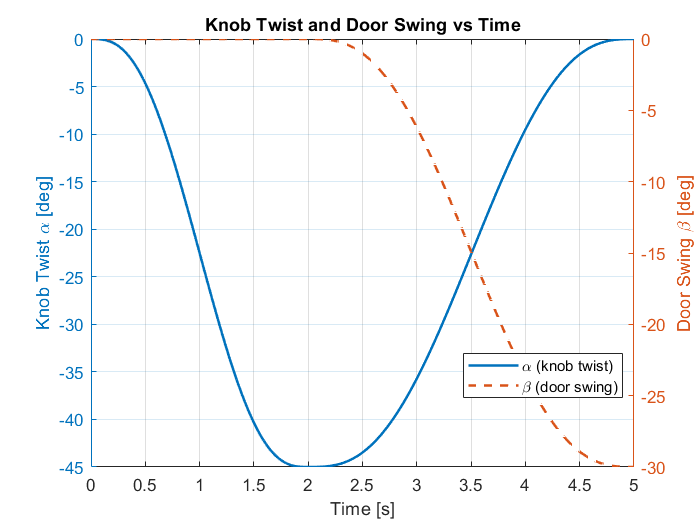
\includegraphics[width=\linewidth]{PartA_Door_Swing.png}
        \caption{Γωνίες στρέψης πομόλου $\alpha(t)$ και περιστροφής πόρτας $\beta(t)$.}
        \label{fig:angle_profiles}
    \end{minipage}
    \hfill
\end{figure}

\vspace{0.2cm}

\subsection{Ανάλυση Αποτελεσμάτων}

Από την ανάλυση των παραπάνω διαγραμμάτων προκύπτουν τα εξής:

\begin{itemize}
    \item \textbf{Θέση πομόλου}: Παρατηρείται ότι η $z_h$ διατηρείται σταθερή καθ’ όλη τη διάρκεια, επιβεβαιώνοντας πως δεν υπάρχει κατακόρυφη μετατόπιση. Η $x_h$ εμφανίζει μικρή μεταβολή κατά την επαναφορά, ενώ η $y_h$ μειώνεται σημαντικά μετά το πέρας της στρέψης, φανερώνοντας τη μετακίνηση της πόρτας προς τα πίσω.
    
    \item \textbf{Προσανατολισμός πομόλου}: Οι καμπύλες $q_0$ έως $q_3$ μεταβάλλονται ομαλά, χωρίς ασυνέχειες ή απότομες μεταβολές, επιβεβαιώνοντας σωστή κινηματική αναπαράσταση της περιστροφής του πομόλου μέσω μοναδιαίου τεταρτογωνίου.

    \item \textbf{Γωνιακά προφίλ $\alpha(t)$ και $\beta(t)$}: Το μοντέλο ακολουθεί πιστά το κινηματικό σενάριο. Πρώτα ολοκληρώνεται η στροφή του πομόλου ($\alpha$), και μόνο τότε ξεκινά το άνοιγμα της πόρτας ($\beta$), κάτι που φαίνεται από τη διακριτή χρονική διαδοχή των γωνιών.

    \item \textbf{Οπτικά στιγμιότυπα}: Απεικονίζουν επιτυχώς την κίνηση του συστήματος σε κρίσιμα χρονικά σημεία. Επιβεβαιώνεται ότι το σύστημα ανταποκρίνεται φυσιολογικά στο σενάριο, χωρίς αριθμητικά σφάλματα ή αντικρουόμενες μετακινήσεις.
\end{itemize}

\hspace{-0.6cm}Η συνολική συμπεριφορά της πόρτας και του πομόλου επιβεβαιώνει την εγκυρότητα του κινηματικού μοντέλου και τη σωστή υλοποίηση των τροχιών και φαίνεται πως ο κώδικας επιλύει ακριβώς το πρόβλημα που ζητήθηκε. Ο αντίστοιχος κώδικας βρίσκεται στο αρχείο \(PartA.m\).

\chapter{Εργασία Ρομποτικής: Τμήμα Β}

\section{Περιγραφή του προβλήματος και απαιτήσεων}

Σε συνέχεια του Τμήματος Α, στο Τμήμα Β της εργασίας εξετάζεται η επίλυση του προβλήματος της αντιστροφικής κινηματικής για τον ρομποτικό βραχίονα \en \texttt{UR10}\gr, προκειμένου να ακολουθήσει την προκαθορισμένη τροχιά του πόμολου \en (handle) \gr που υπολογίστηκε στο Τμήμα Α.

\vspace{0.2cm}

\hspace{-0.6cm}Ο βραχίονας \en \texttt{UR10} \gr διαθέτει 6 βαθμούς ελευθερίας και προσομοιώνεται με χρήση του \en Robotics Toolbox \gr και ο κώδικας του κινηματικού αυτού μοντέλου δόθηκε ως βοήθημα στην υλοποίηση του Τμήματος Β και είναι \(included\) στο ίδιο \(path\) με τον κώδικα \en MATLAB \gr του Τμήματος Β ως \(ur10robot.m\). Στόχος είναι να υπολογιστεί για κάθε χρονική στιγμή το διάνυσμα αρθρώσεων $\mathbf{q}(t) \in \mathbb{R}^6$ το οποίο τοποθετεί το άκρο του ρομπότ \en (end-effector) \gr έτσι ώστε να συμπίπτει με το πλαίσιο $\{H\}$ του πόμολου.

\vspace{0.2cm}

\hspace{-0.6cm}Η χρονική διάρκεια παραμένει $T = 5~\mathrm{s}$ και χρησιμοποιείται η ίδια δειγματοληψία με το Τμήμα Α: $n = 501$ δείγματα, με περίοδο $dt = 0.01~\mathrm{s}$.

\vspace{0.2cm}

\hspace{-0.6cm}Το ρομπότ αρχικά τοποθετείται στη θέση:

\[
\mathbf{q}_0 = [-1.7752,\ -1.1823,\ 0.9674,\ 0.2149,\ 1.3664,\ 1.5708]^\top \ \mathrm{rad}
\]

\hspace{-0.6cm}και η σχετική θέση του άκρου ως προς το πόμολο είναι σταθερή και περιγράφεται με τον μετασχηματισμό \en $g_{he}$ \gr (σταθερό \en hand-eye offset\gr).

\begin{figure}[H]
    \centering
    \includegraphics[width=0.7\textwidth]{ROBOT.png}
    \caption{(α$'$) Απεικόνιση του ρομπότ \en UR10 \gr στην αρχική του θέση με το πλαίσιο του άκρου \{e\}. 
    (β$'$) Σχηματική απεικόνιση του σταθερού μετασχηματισμού $g_{he}$ μεταξύ του πλαισίου του πομόλου \{H\} και του άκρου \{e\}.}
    \label{fig:he_offset}
\end{figure}

\vspace{0.3cm}

\section{Προσέγγιση υλοποίησης σε \en MATLAB \gr}

Ο κώδικας του Τμήματος Β έχει την εξής δομή:

\begin{itemize}
    \item Φόρτωση των τροχιών $g_H(t)$ και $g_D(t)$ από το Τμήμα Α που έχουν αποθηκευτεί ως δεδομένα \en .mat \gr μορφής.
    \item Υλοποίηση επανάληψης αντιστροφικής κινηματικής με χρονικό βήμα $dt$.
    \item Υπολογισμός τροχιάς θέσεων $q(t)$ και ταχυτήτων $\dot{q}(t)$ αρθρώσεων.
    \item Αποθήκευση και απεικόνιση της τελικής τροχιάς του ρομπότ.
\end{itemize}

\vspace{0.2cm}

\subsection{Χρήσιμες εντολές από \en Robotics Toolbox \gr που αξιοποιήθηκαν}

\begin{itemize}
    \item \en \texttt{ur10.fkine(q)}\gr: Υπολογίζει τον ομογενή μετασχηματισμό του άκρου \en (forward kinematics) \gr για τη θέση αρθρώσεων $\mathbf{q}$.
    \item \en \texttt{ur10.jacobe(q)}\gr: Επιστρέφει την Ιακωβιανή πίνακα του άκρου \en (6x6) \gr στο παγκόσμιο σύστημα.
    \item \en \texttt{tr2delta(A, B)}\gr: Υπολογίζει εξαδιάστατο διάνυσμα σφάλματος μετασχηματισμού από $A$ προς $B$ στο χώρο $\mathrm{SE}(3)$.
    \item \en \texttt{pinv(J)}\gr: Υπολογίζει τη ψευδοαντίστροφη του πίνακα $J$, απαραίτητη για την επίλυση υπερπροσδιορισμένων γραμμικών συστημάτων.
    \item \en \texttt{transl(T)}\gr: Εξάγει το διάνυσμα θέσης από ομογενή πίνακα μετασχηματισμού $T$.
    \item \en \texttt{UnitQuaternion(T)}\gr: Μετατρέπει μετασχηματισμό $T \in \mathrm{SE}(3)$ σε μοναδιαίο τεταρτογώνιο \en (quaternion)\gr.
    \item \en \texttt{trplot(T, \dots)}\gr: Γραφική απεικόνιση συστήματος συντεταγμένων του μετασχηματισμού $T$.
    \item \en \texttt{ur10.plot(q)}\gr: Γραφική απεικόνιση του ρομπότ στη θέση $q$ \en (offline rendering)\gr.
    \item \en \texttt{ur10.animate(q)}\gr: Ενημερώνει την κίνηση του ρομπότ δυναμικά \en (real-time animation)\gr.
\end{itemize}

\vspace{0.3cm}

\section{Ενδελεχής ανάλυση και μεθοδολογία επίλυσης}

Το πρόβλημα του Τμήματος B όπως προαναφέρθηκε αφορά την υλοποίηση της αντιστροφής κινηματικής για έναν ρομποτικό βραχίονα \en UR10\gr, με σκοπό να εκτελέσει την επιθυμητή τροχιά του πομόλου όπως αυτή προδιαγράφηκε στο Τμήμα A. Η επίλυση υλοποιείται με τη χρήση της Ιακωβιανής του άκρου \en (Jacobian-based IK)\gr, με έμφαση στην αριθμητική συνέπεια και την σταθερότητα της λύσης.

\vspace{0.2cm}

\subsection{Δομή του αλγορίθμου}

Η αντιστροφή κινηματικής εφαρμόζεται για κάθε χρονική στιγμή $t_k$, με στόχο να υπολογιστεί μια ακολουθία γωνιών αρθρώσεων $\mathbf{q}_k$ που να ικανοποιεί την επιθυμητή θέση και προσανατολισμό του άκρου. Για τον σκοπό αυτό χρησιμοποιούνται τα εξής:

\begin{itemize}
    \item Η επιθυμητή τροχιά του πομόλου $g_H(t)$, προερχόμενη από το Τμήμα Α.
    \item Ο σταθερός μετασχηματισμός \textit{\en hand–eye\gr} $g_{he}$ μεταξύ του άκρου του ρομπότ και του πομόλου.
    \item Η αριθμητική Ιακωβιανή $J$ του άκρου στο παγκόσμιο πλαίσιο.
\end{itemize}

Ο επιθυμητός μετασχηματισμός του άκρου είναι:

\[
g_e^{\text{\en des\gr}}(t) = g_H(t) \cdot g_{he}
\]

\vspace{0.2cm}

\subsection{Αριθμητική προσέγγιση μέσω διαφορικών σχέσεων}

Η αριθμητική διαδικασία βασίζεται στην εξίσωση του σφάλματος:

\[
\Delta T_k = \text{\en tr2delta\gr}(g_e^{\text{\en curr\gr}}(t_k),~g_e^{\text{\en des\gr}}(t_k)) \in \mathbb{R}^6
\]

\hspace{-0.6cm}η οποία αποδίδει ένα εξαδιάστατο σφάλμα (3 για θέση, 3 για προσανατολισμό).

\hspace{-0.6cm}Ακολούθως, εφαρμόζεται η σχέση:

\[
\dot{\mathbf{q}}_k = J^\dagger(\mathbf{q}_k) \cdot \frac{\Delta T_k}{dt}
\]

\hspace{-0.6cm}όπου $J^\dagger$ είναι η ψευδοαντίστροφη της Ιακωβιανής.

\hspace{-0.6cm}Η ενημέρωση της θέσης αρθρώσεων γίνεται με μέθοδο \en Euler\gr:

\[
\mathbf{q}_{k+1} = \mathbf{q}_k + \dot{\mathbf{q}}_k \cdot dt
\]

\vspace{0.2cm}

\subsection{Προεπεξεργασία και αρχικές συνθήκες}

Το πρόγραμμα αρχικοποιείται με:

\begin{itemize}
    \item $q_0$: Αρχική θέση του \en UR10 \gr ώστε να βρίσκεται κοντά στο πόμολο.
    \item Δειγματοληψία: $n = 501$ χρονικά σημεία με $dt = 0.01~\mathrm{s}$ και $T = 5~\mathrm{s}$.
\end{itemize}

\hspace{-0.6cm}Οι μετασχηματισμοί $g_H(t)$ και $g_D(t)$ φορτώνονται από αρχεία που παράχθηκαν στο Τμήμα Α. Το $g_{he}$ είναι σταθερός μετασχηματισμός καθορισμένος ως:

\[
g_{he} =
\begin{bmatrix}
0 & 0 & -1 & 0.1 \\
0 & 1 & 0 & 0.1 \\
1 & 0 & 0 & 0 \\
0 & 0 & 0 & 1
\end{bmatrix}
\]

\vspace{0.2cm}

\subsection{Σημεία ενδιαφέροντος στον κώδικα \en MATLAB\gr}

Η κάθε χρονική στιγμή περιλαμβάνει τα εξής βήματα (έχει προσθεθεί και ψευδοκώδικας για σαφήνεια):

\begin{enumerate}
    \item Υπολογισμός του επιθυμητού μετασχηματισμού: \texttt{\en g\_e\_des = g\_H(:,:,k) * g\_he \gr}
    \item Υπολογισμός του παρόντος μετασχηματισμού: \texttt{\en g\_e\_curr = ur10.fkine(q)\gr}
    \item Υπολογισμός σφάλματος: \texttt{\en deltaT = tr2delta(g\_e\_curr.T, g\_e\_des\gr)}
    \item Υπολογισμός Ιακωβιανής: \texttt{\en J = ur10.jacobe(q)\gr}
    \item Λύση κινηματικής: \texttt{\en q\_dot = pinv(J) * (deltaT / dt)} \gr
    \item Ενημέρωση αρθρώσεων: \texttt{\en q = q + q\_dot * dt} \gr
\end{enumerate}

\vspace{0.2cm}

\subsection{Αποτελέσματα Κώδικα}

Η προσομοίωση παράγει τις παρακάτω τροχιές:

\begin{itemize}
    \item $q(t)$: Θέσεις αρθρώσεων \en UR10 \gr (6 διαστάσεων).
    \item $\dot{q}(t)$: Ταχύτητες αρθρώσεων.
    \item $p_e(t), q_e(t)$: Θέση και προσανατολισμός του άκρου.
    \item $p_{eh}(t), q_{eh}(t)$: Σχετική θέση και προσανατολισμός του άκρου ως προς το πόμολο.
\end{itemize}

\hspace{-0.6cm}Οι τροχιές είναι συνεχείς και ομαλές, επιτυγχάνοντας επιτυχή επίλυση του προβλήματος.

\vspace{0.2cm}

\subsection{Μαθηματική σύνοψη}

Ο συνολικός αλγόριθμος μπορεί να συνοψιστεί ως:

\[
\begin{aligned}
& g_e^{\text{\en des\gr}}(t) = g_H(t) \cdot g_{he} \\
& \Delta T = \text{\en tr2delta\gr}(g_e^{\text{\en curr\gr}}, g_e^{\text{\en des\gr}}) \\
& \dot{\mathbf{q}} = J^\dagger \cdot \frac{\Delta T}{dt} \\
& \mathbf{q}(t+\Delta t) = \mathbf{q}(t) + \dot{\mathbf{q}} \cdot dt
\end{aligned}
\]

\hspace{-0.6cm}Η επίλυση ανήκει στον χώρο των μεθόδων αντιστροφής κινηματικής με χρήση διαφορικών σχέσεων και προσαρμοστικών τεχνικών σε πραγματικό χρόνο, και βασίζεται αρκετά στη δυναμική του \en \texttt{Robotics Toolbox}\gr.

\vspace{0.3cm}

\section{Παρατηρήσεις και Αποτελέσματα}

Στην παρούσα ενότητα παρουσιάζονται και αναλύονται τα αποτελέσματα της προσομοίωσης για το Τμήμα Β, όπου έγινε χρήση αντιστροφικής κινηματικής για τον βραχίονα \en \texttt{UR10} \gr ώστε να ακολουθήσει το πλαίσιο του πομόλου \{H\} σε όλη τη διάρκεια της τροχιάς.

\vspace{0.2cm}

\subsection{Αρχικές Συνθήκες Συστήματος}

Ακολουθούν δύο όψεις της αρχικής θέσης του συστήματος:

\begin{figure}[H]
    \centering
    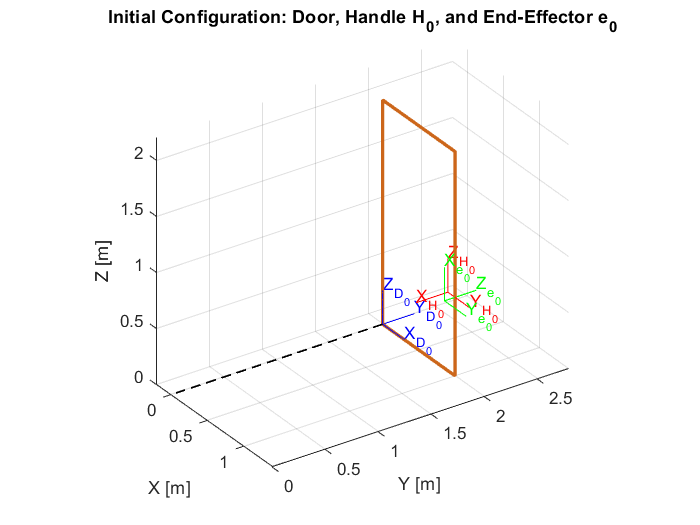
\includegraphics[width=0.48\textwidth]{Part_B_Initial_Conditions_First.png}
    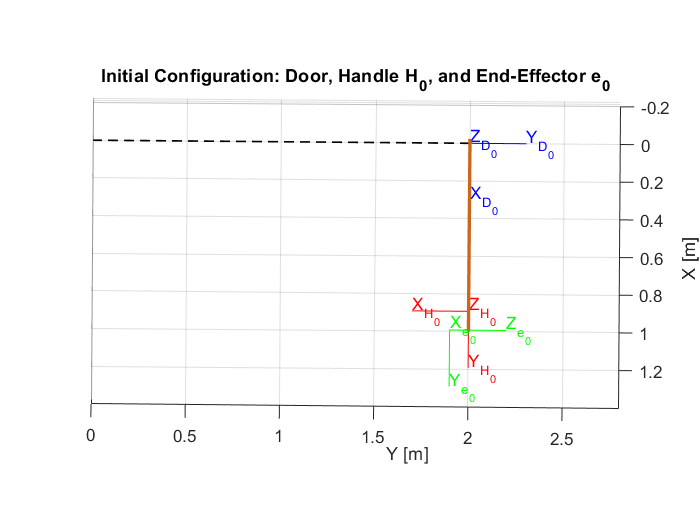
\includegraphics[width=0.48\textwidth]{Part_B_Initial_Conditions_Second.png}
    \caption{Απεικόνιση αρχικής θέσης του ρομπότ, της πόρτας και του πομόλου. Αριστερά: τρισδιάστατη προβολή, δεξιά: προβολή στο επίπεδο \en XY\gr.}
\end{figure}

\vspace{0.2cm}

\subsection{Στιγμιότυπα Κίνησης Ρομπότ, Πόρτας και Πομόλου}

Παρουσιάζονται χαρακτηριστικά στιγμιότυπα της εξέλιξης του ρομπότ και του συστήματος:

\begin{figure}[H]
    \centering
    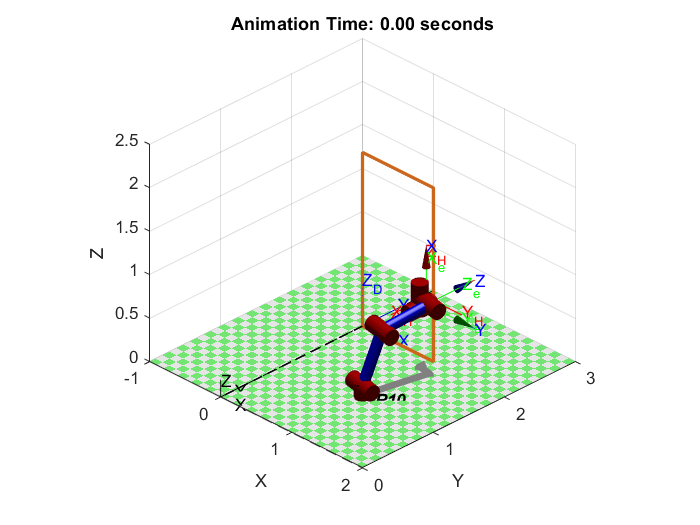
\includegraphics[width=0.48\textwidth]{Part_B_First.png}
    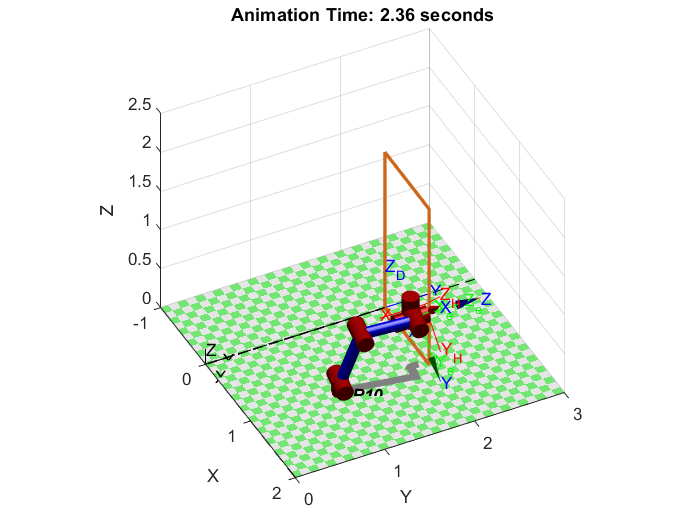
\includegraphics[width=0.48\textwidth]{Part_B_Second.png}
    \caption{Αριστερά: \en t = 0.00s \gr, αρχική θέση \en UR10\gr. Δεξιά: \en t ≈ 2.36s \gr, ολοκλήρωση στρέψης πομόλου.}
\end{figure}

\begin{figure}[H]
    \centering
    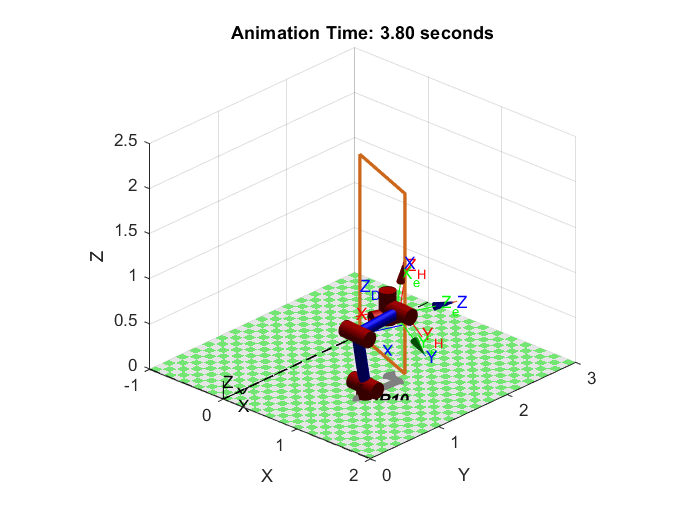
\includegraphics[width=0.48\textwidth]{Part_B_Third.png}
    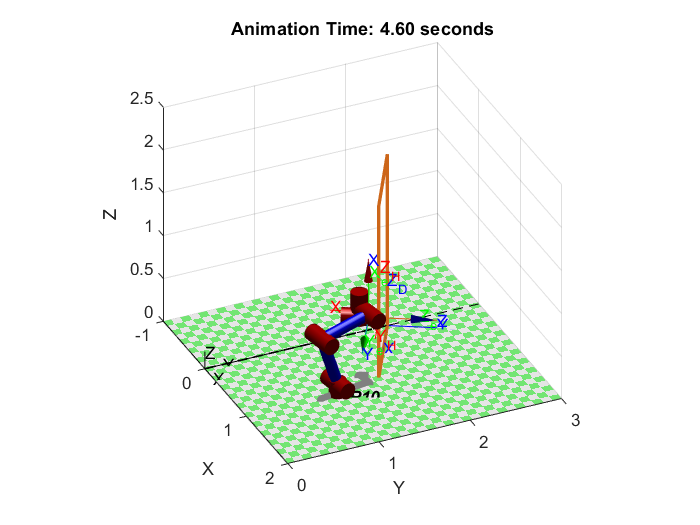
\includegraphics[width=0.48\textwidth]{Part_B_Fourth.png}
    \caption{Αριστερά: \en t ≈ 3.80s\gr, εν εξελίξει άνοιγμα πόρτας. Δεξιά: \en t ≈ 4.60s\gr, κοντά στο τελικό άνοιγμα.}
\end{figure}

\begin{figure}[H]
    \centering
    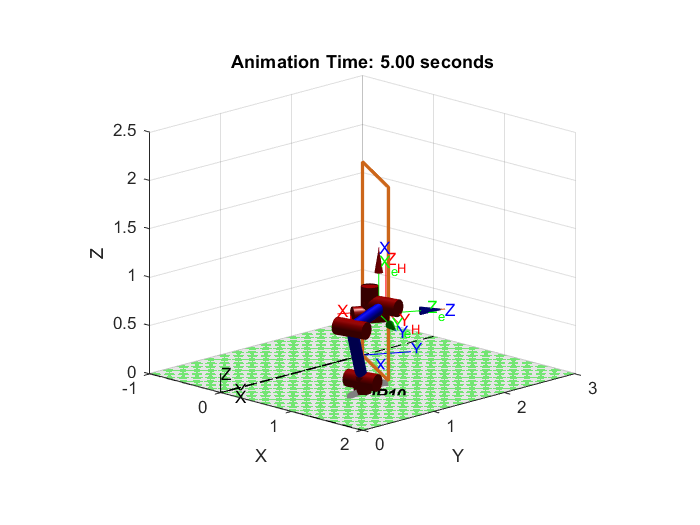
\includegraphics[width=0.48\textwidth]{Part_B_Fifth.png}
    \caption{Τελική φάση: \en t = 5.00s \gr με πλήρως ανοιχτή πόρτα και συνεχή επαφή του \en UR10 \gr με το πλαίσιο \{H\}.}
\end{figure}

\vspace{0.2cm}

\subsection{Διαγράμματα Τροχιών και Αξιολόγησης Κίνησης}

\begin{figure}[H]
    \centering
    \begin{minipage}{0.48\textwidth}
        \centering
        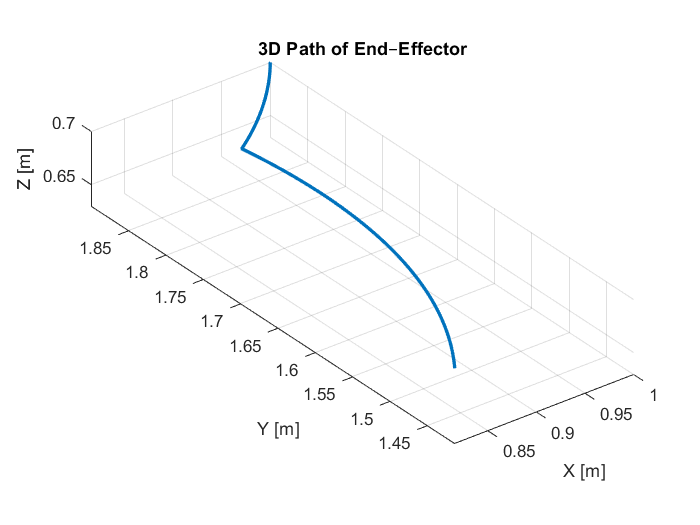
\includegraphics[width=\linewidth]{Part_B_End_Effector_Position.png}
        \caption{Τρισδιάστατη τροχιά του άκρου \en (end–effector) \gr κατά την εκτέλεση της κίνησης. Παρατηρείται συνεχής και λεία μετατόπιση.}
    \end{minipage}
    \hfill
    \begin{minipage}{0.48\textwidth}
        \centering
        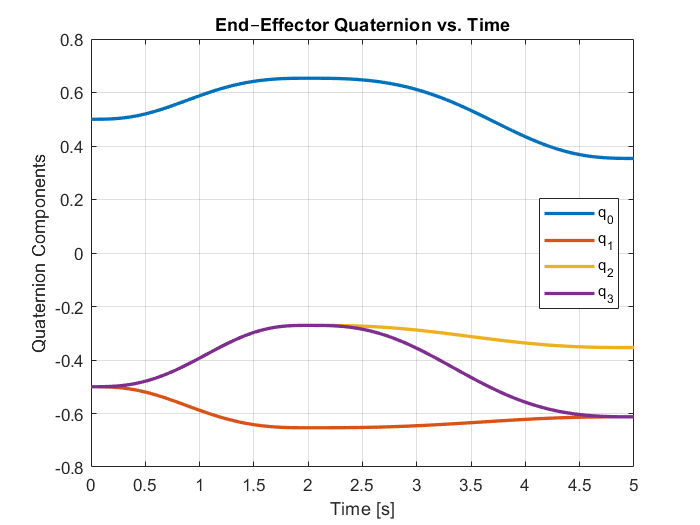
\includegraphics[width=\linewidth]{Part_B_End_Effect_Orientation.png}
        \caption{Συνιστώσες του μοναδιαίου τεταρτογωνίου προσανατολισμού του άκρου. Η ομαλή μεταβολή επιβεβαιώνει σωστή περιστροφή.}
    \end{minipage}
\end{figure}

\vspace{0.3cm}

\begin{figure}[H]
    \centering
    \begin{minipage}{0.48\textwidth}
        \centering
        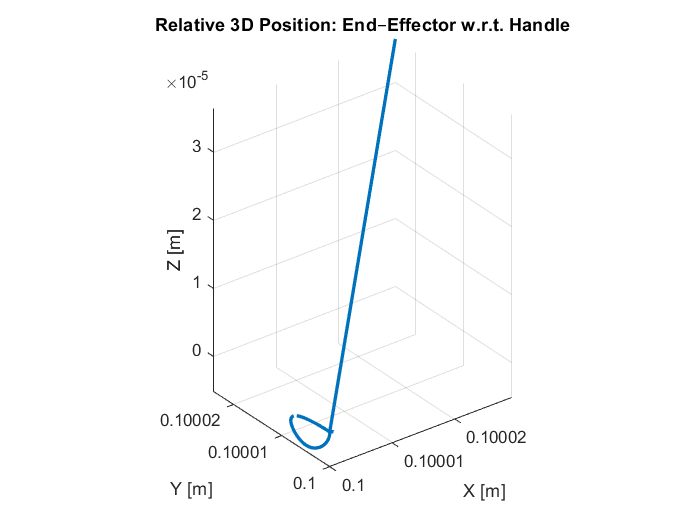
\includegraphics[width=\linewidth]{Part_B_Relative_Position_Handle.png}
        \caption{Σχετική θέση του άκρου ως προς το πλαίσιο του πομόλου \{H\}. Η τροχιά κυμαίνεται σε τάξη $10^{-5}$, επιβεβαιώνοντας ακρίβεια.}
    \end{minipage}
    \hfill
    \begin{minipage}{0.48\textwidth}
        \centering
        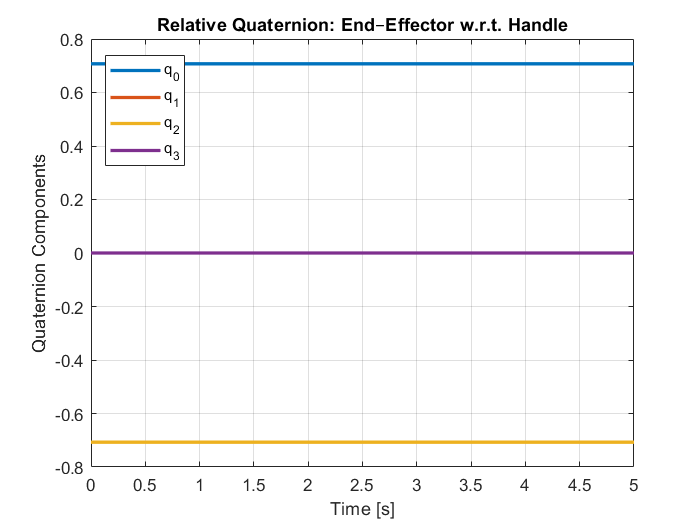
\includegraphics[width=\linewidth]{Part_B_Relative_Orientation.png}
        \caption{Σχετικός προσανατολισμός: ο τεταρτογωνικός προσανατολισμός παραμένει πρακτικά σταθερός, αποδεικνύοντας σταθερότητα σύνδεσης.}
    \end{minipage}
\end{figure}

\vspace{0.3cm}

\begin{figure}[H]
    \centering
    \begin{minipage}{0.48\textwidth}
        \centering
        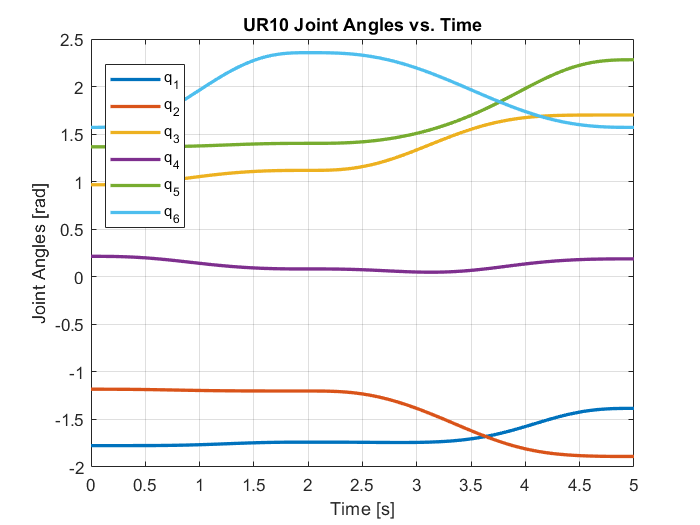
\includegraphics[width=\linewidth]{Part_B_Joint_Positions.png}
        \caption{Χρονική εξέλιξη των γωνιών αρθρώσεων του \en UR10\gr. Όλες οι τροχιές είναι λείες και συνεχείς, με ρεαλιστικά προφίλ.}
    \end{minipage}
    \hfill
    \begin{minipage}{0.48\textwidth}
        \centering
        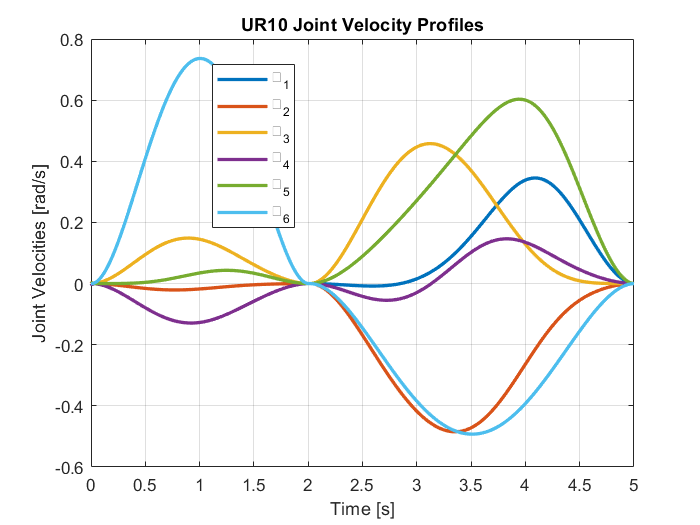
\includegraphics[width=\linewidth]{Part_B_Joint_Velocities.png}
        \caption{Ταχύτητες αρθρώσεων: οι μεταβολές παραμένουν ομαλές, χωρίς απότομες αλλαγές που θα έθεταν σε κίνδυνο τον ελεγκτή.}
    \end{minipage}
\end{figure}

\vspace{0.4cm}

\subsection{Ανάλυση Αποτελεσμάτων}

Από την παρατήρηση των διαγραμμάτων και στιγμιοτύπων, προκύπτουν οι ακόλουθες παρατηρήσεις:

\begin{itemize}
    \item \textbf{Διατήρηση επαφής με το πλαίσιο \{H\}}: Το γράφημα της σχετικής θέσης του άκρου δείχνει μεταβολές στην τάξη του $10^{-5}$, δηλαδή κάτω από χιλιοστά, γεγονός που αποδεικνύει ότι το άκρο ακολουθεί με απόλυτη ακρίβεια την τροχιά του πομόλου.

    \item \textbf{Σταθερότητα στον προσανατολισμό}: Η διατήρηση σταθερού τεταρτογωνίου στον σχετικό προσανατολισμό του άκρου ως προς το \{H\} επιβεβαιώνει την επιτυχή σταθεροποίηση του \en \textit{hand–eye} offset \gr σε όλη τη διάρκεια της κίνησης.

    \item \textbf{Ομαλότητα τροχιών}: Οι γωνίες αρθρώσεων και οι ταχύτητες παρουσιάζουν φυσική και συνεχή εξέλιξη, όπως απαιτείται για ρομποτικά συστήματα που αλληλεπιδρούν με περιβάλλον.

    \item \textbf{Οπτική τεκμηρίωση κίνησης}: Από τα χρονικά στιγμιότυπα του ρομπότ επιβεβαιώνεται ότι η τροχιά ακολουθεί επακριβώς την πορεία του πομόλου, ενώ το ρομπότ τροποποιεί στάση χωρίς απώλεια σταθερότητας.

    \item \textbf{Πιστότητα αντιστροφικής κινηματικής}: Η λύση του προβλήματος μέσω ψευδοαντίστροφης Ιακωβιανής αποδεικνύεται επαρκής, προσφέροντας ακριβή παρακολούθηση χωρίς αριθμητικά φαινόμενα όπως ιδιομορφίες ή ασυνέχειες.
\end{itemize}

\noindent Συμπερασματικά, η αριθμητική προσέγγιση αντιστροφικής κινηματικής υλοποιείται επιτυχώς, με τη χρήση εργαλείων του \en \texttt{Robotics Toolbox}\gr και τον κώδικα του αρχείου \(PartB.m\) ενώ οι αρχικές συνθήκες του συστήματος στατικά προκύπτουν στο αρχείο \(debug.m\).


\bibliographystyle{plain}
\begin{thebibliography}{1}
    \bibitem{first_bibl}
    \en https://elearning.auth.gr/pluginfile.php/526639/mod\_resource/content/1/ur10robot.m
    \bibitem{second_bibl}
    \en https://petercorke.com/toolboxes/robotics-toolbox/
\end{thebibliography}

\end{document}